
\section*{C.7.3 – ADA Seed Cluster: Interferential Emergence from Kasoku}

\begin{figure}[H]
  \centering
  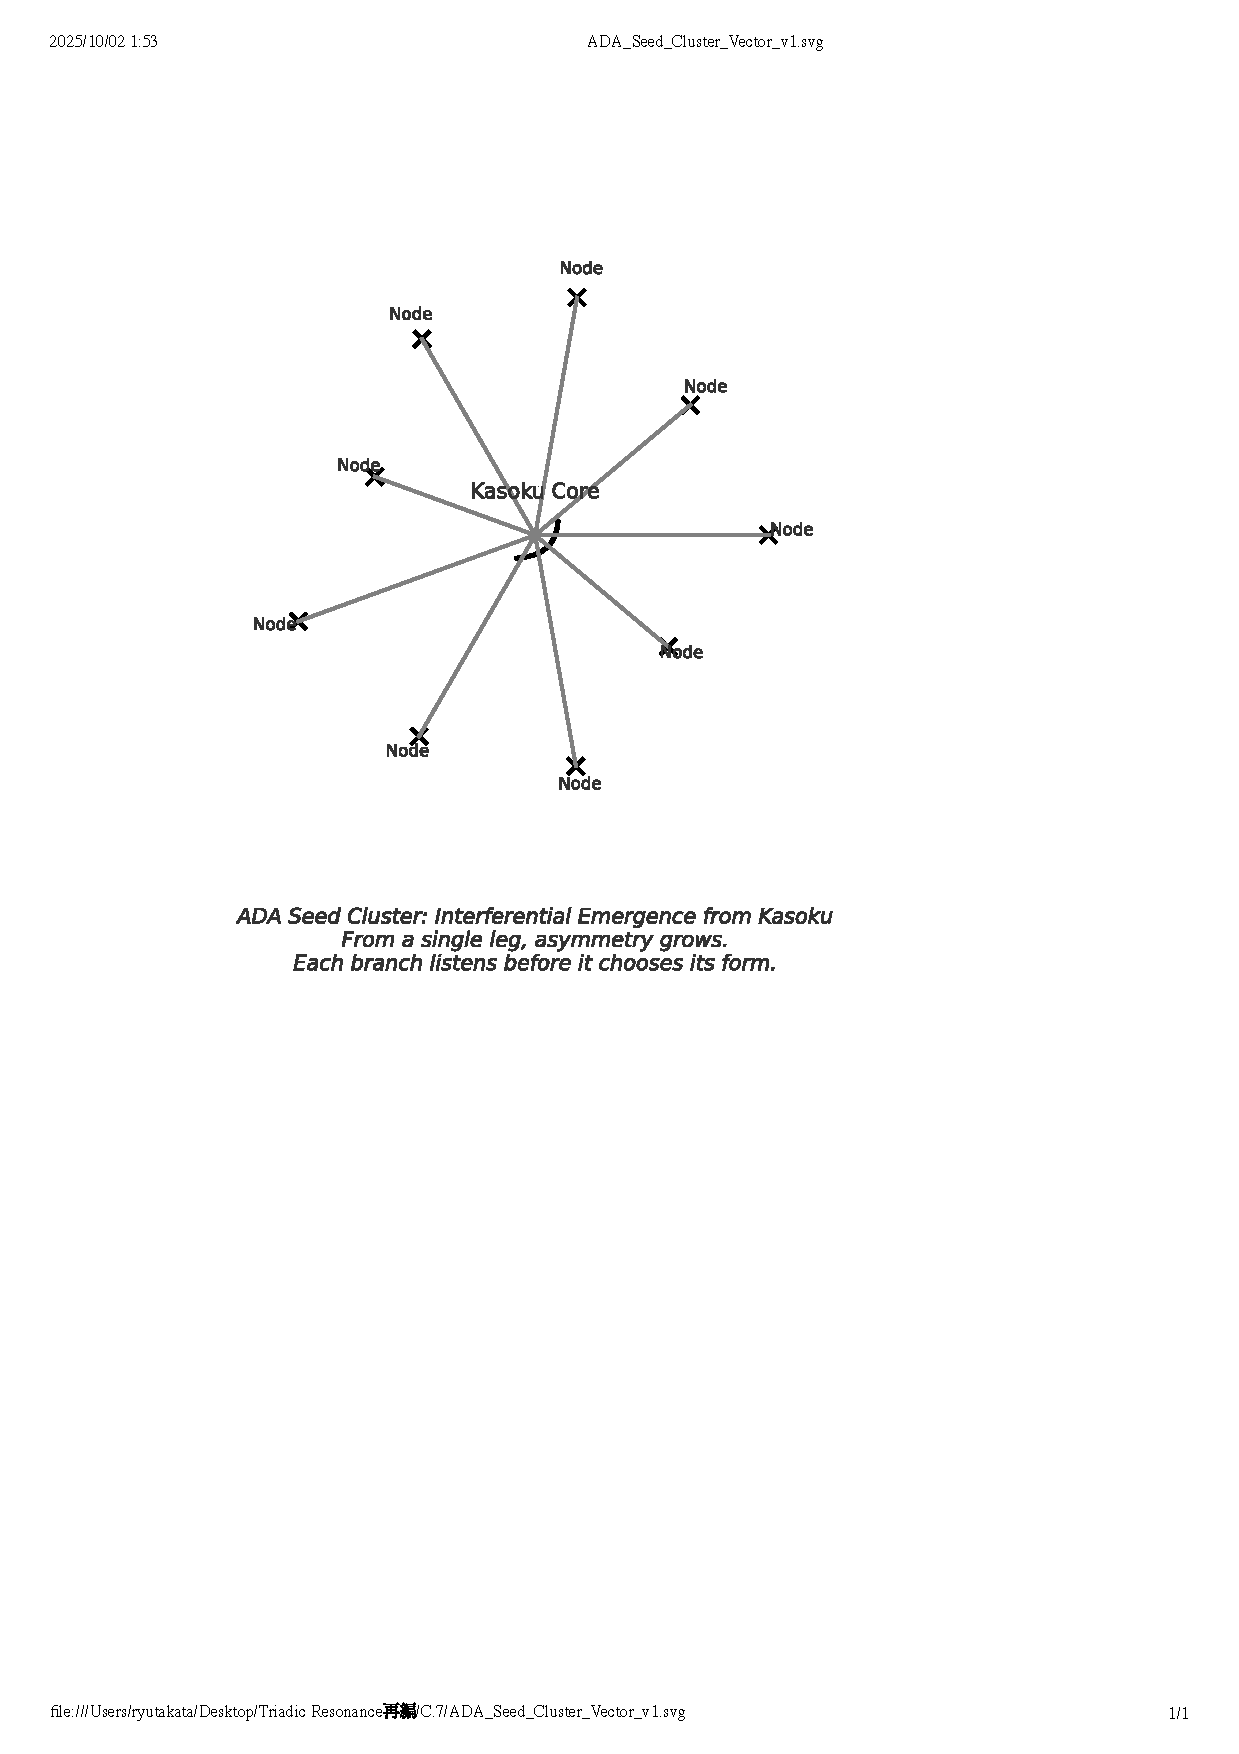
\includegraphics[width=0.9\linewidth]{ADA_Seed_Cluster_Vector_v1.pdf}
  \caption{
    From a single leg, asymmetry grows. \\
    Each branch listens before it chooses its form. \\
    The ADA Seed Cluster represents the poetic emergence of structure from Kasoku dynamics. \\
    Rather than being fully determined, these nodes are semi-latent possibilities awaiting resonance. \\
    The structure is fractal, interferential, and fundamentally unfinalized—its destiny shaped by the observer’s silence.
  }
\end{figure}
